\chapter{Big Data Architectures}

\section{Introduzione alle Architetture Big Data}

Un'architettura Big Data è progettata per gestire l'ingestione, l'elaborazione e l'analisi di dati che risultano troppo grandi o complessi per i sistemi di database tradizionali. 

Le soluzioni Big Data tipicamente coinvolgono una o più delle seguenti tipologie di carico di lavoro (workload):
\begin{itemize}
    \item \textbf{Batch processing} di sorgenti Big Data \textit{at rest} (dati a riposo/archiviati).
    \item \textbf{Real-time processing} di Big Data \textit{in motion} (dati in movimento/streaming).
    \item \textbf{Interactive exploration} (esplorazione interattiva) dei Big Data.
    \item \textbf{Predictive analytics e machine learning}.
\end{itemize}

\subsection{Quando utilizzare un'architettura Big Data}
È opportuno considerare l'adozione di un'architettura Big Data quando si ha la necessità di:
\begin{itemize}
    \item Memorizzare ed elaborare dati in \textbf{volumi troppo ampi} per un database tradizionale.
    \item Trasformare \textbf{dati non strutturati} per finalità di analisi e reportistica.
    \item Catturare, elaborare e analizzare \textbf{flussi illimitati di dati (unbounded streams)} in tempo reale o con bassa latenza (low latency).
\end{itemize}

\begin{remark}[Nota del professore: Scegliere lo strumento giusto]
Il professore sottolinea un aspetto fondamentale per un ingegnere: è cruciale utilizzare la soluzione corretta per il problema specifico che si deve risolvere. Non bisogna adottare un framework Big Data solo perché "lo fanno tutti" o perché è una tecnologia di tendenza, specialmente se i dati da gestire sono di piccole dimensioni. Utilizzare un'architettura complessa quando non è necessaria porta unicamente a uno spreco di tempo e di risorse computazionali.
\end{remark}

\section{La Lambda Architecture}

L'architettura Big Data più frequentemente utilizzata (secondo il professore, presente in circa il 99\% dei sistemi basati su framework Big Data) è la \textbf{Lambda Architecture}. È stata proposta per la prima volta da Nathan Marz nel 2011 e, seppur basata su idee molto semplici, risulta estremamente efficace ed efficiente.

\subsection{Definizioni a confronto}
Per comprendere appieno questa architettura, è utile analizzare tre diverse definizioni fornite in letteratura e nel settore industriale:

\begin{definition}[Definizione \#1 - Nathan Marz]
I database NoSQL (come Cassandra) ottengono la loro scalabilità offrendo un \textbf{modello di dati molto più limitato} rispetto al classico SQL, rendendo complessa l'adattabilità delle applicazioni. Inoltre, essendo database mutabili, \textbf{non sono tolleranti agli errori umani (human-fault tolerant)}. 
La Lambda Architecture nasce dall'uso intelligente e congiunto di diversi strumenti (sistemi di calcolo su larga scala e database) per produrre sistemi scalabili per problemi di dati arbitrari, garantendo la tolleranza agli errori umani con il minimo della complessità.
\end{definition}

\begin{definition}[Definizione \#2 - Databricks]
La Lambda Architecture è un modo per elaborare quantità massive di dati fornendo accesso sia a metodi di \textbf{batch-processing} che di \textbf{stream-processing} attraverso un \textbf{approccio ibrido}. È utilizzata per risolvere il problema del calcolo di funzioni arbitrarie.
\end{definition}

\begin{definition}[Definizione \#3 - Wikipedia]
È un'architettura di elaborazione dati progettata per gestire quantità massive di dati sfruttando i vantaggi sia dei metodi batch che stream. Cerca di \textbf{bilanciare latenza, throughput e tolleranza ai guasti (fault-tolerance)} in questo modo:
\begin{itemize}
    \item Il \textit{batch processing} fornisce viste accurate e complete sui dati archiviati (batch data).
    \item Lo \textit{stream processing} in tempo reale fornisce viste sui dati online.
\end{itemize}
Gli output di queste due viste vengono poi uniti (joined) prima della presentazione finale all'utente.
\end{definition}

\subsection{Il Modello dei Dati nella Lambda Architecture}
La Lambda Architecture si basa fortemente su un modello di dati specifico: utilizza una \textbf{sorgente dati immutabile e append-only} che funge da sistema di registrazione (system of record). 

È pensata per l'ingestione e l'elaborazione di \textbf{eventi dotati di timestamp}, i quali vengono accodati (appended) agli eventi esistenti piuttosto che sovrascriverli. Lo stato del sistema viene determinato dal naturale ordinamento temporale dei dati. 

% FIGURA DA INSERIRE QUI
% Fonte: Slide / Spiegazione a lezione (Intorno a 01:50:11 e 02:09:28 della trascrizione)
% Descrizione: Diagramma strutturale a livelli della Lambda Architecture che mostra il flusso dei dati (Input Data), il layer batch, il layer di speed/streaming e il layer di serving.
\begin{figure}[H]
    \centering
    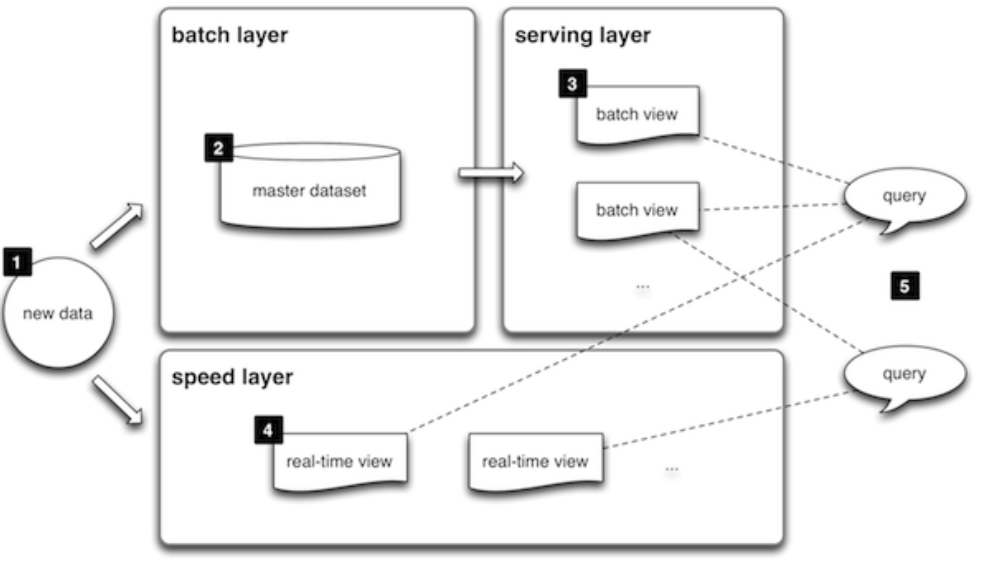
\includegraphics[width=0.8\textwidth]{capitoli/02_Architectures/images/lambda_architecture_diagram.png}
    \caption{Struttura e livelli della Lambda Architecture.}
    \label{fig:lambda_architecture}
\end{figure}

\subsection{Requisiti dell'Architettura}
La Lambda Architecture è progettata per soddisfare i seguenti requisiti fondamentali:

\begin{itemize}
    \item \textbf{Tolleranza ai guasti (Fault-tolerance):} Deve resistere sia ai guasti hardware (hardware failures) sia agli errori umani (human errors).
    \item \textbf{Supporto per molteplici casi d'uso:} Deve gestire sia interrogazioni a bassa latenza sia aggiornamenti complessi sui dati storici.
    \item \textbf{Capacità di Linear Scale-out:} Deve poter scalare orizzontalmente in modo lineare.
\end{itemize}

\begin{remark}[Implementazione dello Scale-out]
Come specificato dal professore, la scalabilità "scale-out" (ovvero l'aggiunta di nuovi nodi al cluster anziché il potenziamento del singolo nodo) viene implementata utilizzando framework e tecnologie progettate nativamente per questo scopo, come i database NoSQL e i framework Hadoop o Spark. Quando si processano dati nel livello batch, si effettua tipicamente un \textit{full scan} (scansione completa) dell'intera collezione di dati in input, analizzando un record alla volta per ottenere il risultato finale.
\end{remark}